\section{Results and Analysis}
\label{sec:results}

% Generated by analysis_outputs/judge_uncertainty/build_random_arm_table.py
% Requires \usepackage{booktabs} and \usepackage[table,dvipsnames]{xcolor}.
\begin{table*}[t]
\centering
\small
\setlength{\tabcolsep}{3.6pt}
\begin{tabular}{lccccccccccccccc}
\toprule
 & \multicolumn{5}{c}{BEETLE UQ} & \multicolumn{5}{c}{SciEntsBank UQ} & \multicolumn{5}{c}{SciEntsBank UD} \\
\cmidrule(lr){2-6}\cmidrule(lr){7-11}\cmidrule(lr){12-16}
Synthetic amount & 1$\times$ & 2$\times$ & 3$\times$ & 4$\times$ & 5$\times$ & 1$\times$ & 2$\times$ & 3$\times$ & 4$\times$ & 5$\times$ & 1$\times$ & 2$\times$ & 3$\times$ & 4$\times$ & 5$\times$ \\
\midrule
w/o synthetic data & \multicolumn{5}{c}{61.2} & \multicolumn{5}{c}{56.5} & \multicolumn{5}{c}{53.8} \\
\midrule
Prompting & $-$0.3 & \cellcolor{BrickRed!18}$-$3.2 & \cellcolor{BrickRed!26}$-$4.5 & \cellcolor{BrickRed!35}$-$6.3 & \cellcolor{BrickRed!36}$-$6.4 & \cellcolor{BrickRed!16}$-$2.8 & \cellcolor{BrickRed!15}$-$2.7 & \cellcolor{BrickRed!18}$-$3.1 & \cellcolor{BrickRed!17}$-$3.0 & \cellcolor{BrickRed!24}$-$4.3 & \cellcolor{BrickRed!18}$-$3.2 & \cellcolor{BrickRed!25}$-$4.5 & \cellcolor{BrickRed!24}$-$4.3 & \cellcolor{BrickRed!25}$-$4.4 & \cellcolor{BrickRed!30}$-$5.4 \\
SFT & \cellcolor{Cerulean!5}+0.9 & \cellcolor{Cerulean!5}+0.9 & \cellcolor{Cerulean!11}+2.0 & \cellcolor{Cerulean!6}+1.1 & \cellcolor{Cerulean!8}+1.4 & \cellcolor{Cerulean!3}+0.5 & \cellcolor{Cerulean!6}+1.1 & \cellcolor{Cerulean!17}+3.0 & \cellcolor{Cerulean!13}+2.4 & \cellcolor{Cerulean!10}+1.9 & \cellcolor{Cerulean!18}+3.1 & \cellcolor{Cerulean!25}+4.4 & \cellcolor{Cerulean!24}+4.3 & \cellcolor{Cerulean!23}+4.0 & \cellcolor{Cerulean!24}+4.3 \\
SFT+DPO & +0.4 & \cellcolor{Cerulean!4}+0.8 & \cellcolor{Cerulean!8}+1.4 & \cellcolor{Cerulean!7}+1.2 & \cellcolor{Cerulean!11}+1.9 & \cellcolor{Cerulean!7}+1.3 & \cellcolor{Cerulean!9}+1.5 & \cellcolor{Cerulean!21}+3.7 & \cellcolor{Cerulean!14}+2.5 & \cellcolor{Cerulean!18}+3.1 & \cellcolor{Cerulean!23}+4.1 & \cellcolor{Cerulean!33}+5.8 & \cellcolor{Cerulean!36}+6.4 & \cellcolor{Cerulean!33}+5.9 & \cellcolor{Cerulean!35}+6.2 \\
DPO & \cellcolor{Cerulean!16}\textbf{+2.8} & \cellcolor{Cerulean!15}\textbf{+2.8} & \cellcolor{Cerulean!17}\textbf{+3.0} & \cellcolor{Cerulean!17}\textbf{+3.1} & \cellcolor{Cerulean!18}\textbf{+3.2} & \cellcolor{Cerulean!35}\textbf{+6.1} & \cellcolor{Cerulean!35}\textbf{+6.2} & \cellcolor{Cerulean!44}\textbf{+7.8} & \cellcolor{Cerulean!45}\textbf{+8.0} & \cellcolor{Cerulean!45}\textbf{+8.0} & \cellcolor{Cerulean!33}\textbf{+5.8} & \cellcolor{Cerulean!36}\textbf{+6.4} & \cellcolor{Cerulean!41}\textbf{+7.2} & \cellcolor{Cerulean!41}\textbf{+7.3} & \cellcolor{Cerulean!39}\textbf{+7.0} \\
\bottomrule
\end{tabular}
\caption{Differences between the performance of the ASAS model with and without synthetic data. \textbf{Bold} marks the best results per column. Each cell is an average of five random draws and four encoders.}
\label{tab:random-arm}
\end{table*}

\subsection{Diversity and Realism of Synthetic Answers}
\label{sec:realism-diversity}
% \noindent\textbf{Are the synthetic answers realistic and diverse enough?}

\vspace{0.5ex}
\noindent\colorbox{gray!15}{\parbox{\dimexpr\linewidth-2\fboxsep\relax}{%
Simple few-shot prompting with LLMs produces less diverse and less realistic answers than fine-tuned synthesizers.}}


\begin{figure}[t]
    \centering
    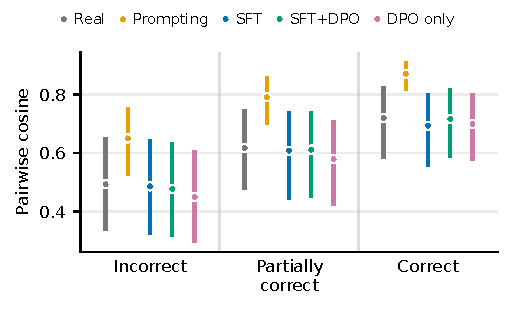
\includegraphics[width=0.8\columnwidth]{fig2_level_similarity_compact.pdf}
    \caption{Pairwise cosine similarity of answers within each correctness level, for real and synthetic answers.}
    \label{fig:level_similarity}
\end{figure}

\begin{figure}[t]
    \centering
    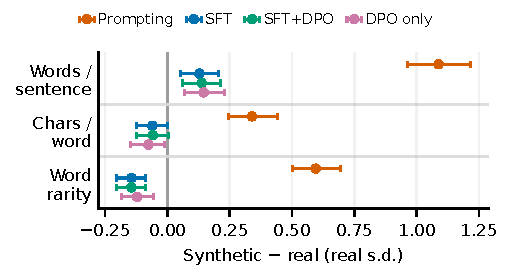
\includegraphics[width=0.8\columnwidth]{semantic_answer_style_metrics_compact.pdf}
    \caption{Difference in answer style metrics between synthetic and real answers. Word rarity is the mean word surprisal, $-\log_{10}$ of the add-half-smoothed word frequency in the benchmark's real training answers; out-of-vocabulary words, including misspellings, receive the maximum value.}
    \label{fig:style_metrics}
\end{figure}
Before using the synthetic answers for training, we first evaluate how \textbf{diverse} and \textbf{realistic} they are, which are crucial for effective data augmentation \citep{kumarDataAugmentationUsing2020,ceginChatGPTReplaceCrowdsourcing2023}. 

\noindent\textbf{Diversity} We measure semantic diversity as the pairwise cosine similarity of sentence embeddings among answers of the same correctness level, and compare it against that of the real answers~(\autoref{fig:level_similarity}). In principle, diversity naturally increases as the correctness level decreases because correct answers tend to be more homogeneous. The answers from the fine-tuned methods closely match the real answers in pairwise similarity across all levels, whereas the prompting method produces answers that are less diverse and more similar to each other.

\noindent\textbf{Realism} We measure realism as how closely the style of the synthetic answers matches that of the real student answers~(\autoref{fig:style_metrics}). For this, we compute the number of words in sentences, the mean number of characters per word, and the mean word rarity. Simply prompting the LLMs produces overly verbose and complex answers that deviate from the style of real student answers, while the fine-tuned synthesizers produce far more realistic answers. However, there is no significant difference among the three fine-tuned methods.

\subsection{Scoring Unseen Questions with Synthetic Answers}
\label{sec:scoring-unseen}

\vspace{0.5ex}
\noindent\colorbox{gray!15}{\parbox{\dimexpr\linewidth-2\fboxsep\relax}{%
Diverse and realistic synthetic student answers improve the performance of ASAS models on unseen questions, with the DPO approach achieving the best results. The positive and negative effects of each synthesizer persist as the amount of synthetic data increases.}}

We then train the ASAS model on the synthetic answers together with the original training data and evaluate it on the unseen questions. The synthetic answers are balanced across questions and levels and randomly sampled five times. By default, they match the size of the original training data, and we increase the amount up to five times this size. \autoref{tab:random-arm} reports the change in macro F1 relative to training on the original data only, and per-model scores are given in \autoref{tab:appendix-random-amount} (\autoref{app:per-model-results}).

At the default amount, prompting does not help and even lowers the macro F1 on SciEntsBank by around 3 points, consistent with its less realistic and less diverse answers (\autoref{sec:realism-diversity}). The three fine-tuned synthesizers improve the macro F1 in all settings, with SFT+DPO slightly ahead of SFT on SciEntsBank. DPO is the best in all three settings, improving the macro F1 by up to 6.1 points on SciEntsBank UQ.

Increasing the amount of synthetic data amplifies these effects. For the fine-tuned synthesizers the gains grow further, with most of the improvement reached at two to three times the original data size, while for prompting the loss keeps growing and reaches 6.4 points on BEETLE UQ at five times the size. This indicates that more realistic synthetic answers translate to better downstream performance, whereas unrealistic ones become more harmful the more of them are added.

Although the three fine-tuned synthesizers produce answers of similar style and diversity~(\autoref{sec:realism-diversity}), DPO method outperforms the others. We attribute the gap to level fidelity: the judge panel, trained only on real answers, assigns DPO answers to their requested level more often than answers from any other synthesizer~(\autoref{tab:judge-f1-by-arm} in~\autoref{app:judge-scorer}). This is consistent with the level-contrastive objective, which explicitly separates adjacent levels, whereas SFT only imitates answers at the requested level. 



\subsection{Judge-Based Selection}

\vspace{0.5ex}
\noindent\colorbox{gray!15}{\parbox{\dimexpr\linewidth-2\fboxsep\relax}{%
Selecting synthetic answers by judge probabilities filters out low-quality answers, and its benefit over random selection grows with the amount of synthetic data.}}


\begin{figure}[t]
    \centering
    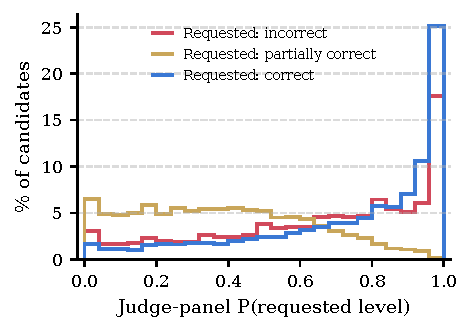
\includegraphics[width=0.8\columnwidth]{fig5_judge_probability.pdf}
    \caption{Distribution of the judge-panel probability $s(a)$ of the requested level, by requested level.}
    \label{fig:judge-probability}
\end{figure}

\begin{figure}[t]
    \centering
    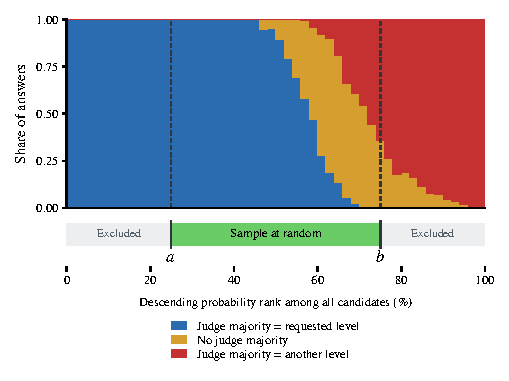
\includegraphics[width=0.8\columnwidth]{judge_hard_vote_group_share.pdf}
    \caption{Share of candidate answers by judge majority outcome, ranked by the panel probability assigned to the requested level.}
    \label{fig:judge-vote-share}
\end{figure}

\begin{figure}[t]
    \centering
    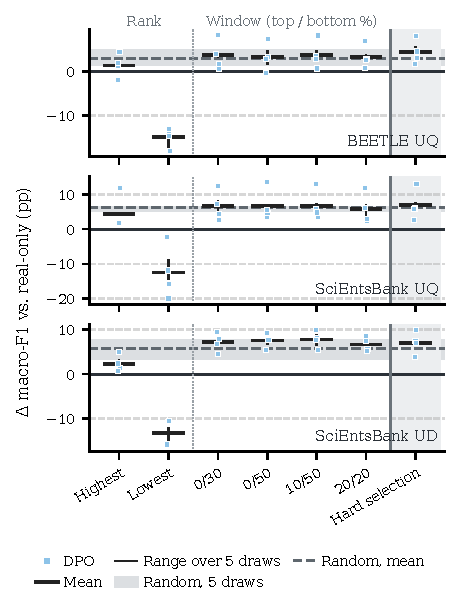
\includegraphics[width=0.8\columnwidth]{fig7_policy_summary_draws.pdf}
    \caption{Change in macro F1 relative to training on real data only for judge-based selection policies and random selection. Points show means and bars show ranges over five draws.}
    \label{fig:selection-policies}
\end{figure}

\begin{figure}[t]
    \centering
    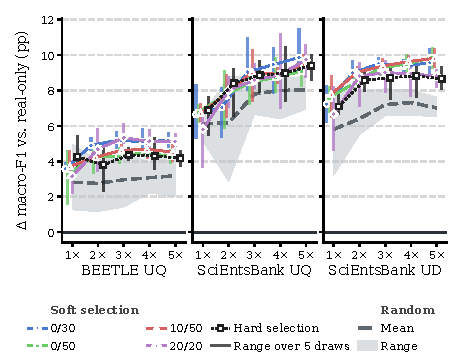
\includegraphics[width=0.8\columnwidth]{fig10_fraction_absolute.pdf}
    \caption{Change in macro F1 relative to training on real data only at different amounts of synthetic data, for judge-based and random selection. Points show means, and bars show ranges over five draws.}
    \label{fig:selection-amount}
\end{figure}
\paragraph{Selection Policies}
Not all generated answers are equally useful or aligned with the intended score level. As \autoref{tab:random-arm} shows, regardless of the synthesizer, the performance plateaus or drops after a certain amount of synthetic data is added. To investigate whether selection by judge probabilities filters high-quality synthetic data, we score each synthetic instance with a panel of judges~(\autoref{sec:selection-training}). Since DPO is the best synthesizer, we experiment only with synthetic answers generated by it. As before, all experiments are repeated five times with different random draws of synthetic answers.



We experiment with different selection policies: 

\begin{itemize}
    \item \textbf{Random selection} The default policy in \autoref{tab:random-arm}. It is used as a baseline.
    \item \textbf{Hard Selection} We select a candidate answer if the majority (more than half) of the judges assign it to the requested level. This is an intuitive policy and serves as the second baseline.
    \item \textbf{Highest-Rank} We first rank the candidates within each question, requested level and generator by their panel score $s(a)$ (Eq.~\eqref{eq:panel-score}), and then select the candidates with the highest scores. These are the candidates that the judges most confidently assign to the requested level.
    \item \textbf{Lowest-Rank} Using the same ranking, we select the candidates with the lowest scores, i.e., those that the judges most confidently assign to another level.
    \item \textbf{Soft Selection} \textit{Hard Selection} and \textit{Highest-Rank} keep only answers that the judges unambiguously place at the requested level. However, the judges are trained only on the original training data and inherit its biases, so answers they are unsure about are not necessarily wrong. To investigate whether such answers help, we use the same ranking and apply a window $(w_{\mathrm{top}}, w_{\mathrm{bot}})$ that excludes its top $w_{\mathrm{top}}\%$ and bottom $w_{\mathrm{bot}}\%$. Both tails are answers on which the judges are confident, but in opposite directions: at the top they agree with the requested level, at the bottom they assign the answer to another level. We sample at random from the remaining candidates, on which the judges are less certain. As \autoref{fig:judge-vote-share} shows, moving the window down the ranking shifts the selected answers from those with a judge majority for the requested level to those without a judge majority, so the choice of $(w_{\mathrm{top}}, w_{\mathrm{bot}})$ controls how many ambiguous answers enter the training data.
\end{itemize}


To balance the amount of synthetic data across questions and levels, the selection policy is applied separately to each question and requested level; otherwise, the selected answers would be dominated by correct and incorrect answers, as the judges are more confident about them~(\autoref{fig:judge-probability}). 

We test four windows: $(w_{\mathrm{top}}, w_{\mathrm{bot}}) \in \{(0, 30), (0, 50), (10, 50), (20, 20)\}$. \autoref{fig:selection-policies} shows the results, and per-model scores are provided in \autoref{tab:appendix-selection-amount} in \autoref{app:per-model-results}. Hard Selection and all four windows perform on par with random selection: their means lie within or at the edge of the range of the five random draws on all three test sets. The exception is Lowest-Rank, which lowers the macro F1 by 12 to 15 points relative to training on real data only. The answers that the judges most confidently assign to another level do harm the scorer, which suggests that the judges reliably identify off-level answers. Highest-Rank also falls below random selection, most clearly on SciEntsBank UD. Keeping only the answers that the judges are most confident about thus does not help either, in line with our motivation for the windows.

Although the effect of selection is small at the default amount of synthetic data, it becomes clear when more synthetic data is added. \autoref{fig:selection-amount} shows that random selection plateaus after two to three times the original data size, and on SciEntsBank UD it even declines slightly afterwards. With judge-based selection, the performance does not plateau in the same way: on SciEntsBank the gains keep growing up to five times the original size, and on BEETLE UQ they rise until three times and then stay well above random selection. At five times, the soft-selection windows are about 1 to 3 points above the mean of random selection on all three test sets, and their means lie above or at the upper edge of the range of random draws. Selection by judge probabilities therefore filters out the answers that stop being useful as the amount grows, so that more synthetic data keeps paying off. Hard Selection benefits less: on BEETLE UQ and SciEntsBank UD it levels off below the best windows, which suggests that the ambiguous answers kept by the windows contribute useful information when many synthetic answers are used. Nevertheless, the gain from adding synthetic data shows diminishing returns: each additional increment of synthetic data improves the scorer by less than the previous one.  


The four windows differ by at most about one point of macro F1 on each test set at the default amount (\autoref{fig:selection-policies}), which is well within the spread across individual draws, so no window is clearly superior. Overall, however, $(0, 30)$ is the best window: it is at or near the top on all three test sets and across the tested amounts. We hypothesize that it allows for a wide range of both \emph{reliable} and \emph{informative} answers while keeping the low-quality ones out. It retains the answers that the judges most confidently place at the requested level, as well as the more ambiguous ones that add variety, and it removes only the bottom 30\%, which Lowest-Rank shows to be harmful.

\subsection{The Role of Synthetic Data in ASAS}
DPO synthesizers trained on real student answers produce realistic answers that improve ASAS, and soft selection adds further gains when more synthetic data is used. Nevertheless, these gains approach a ceiling (\autoref{fig:selection-amount}), and they are obtained by training on real and synthetic answers together. Even the best configuration reaches a macro F1 of only about 65 to 68, depending on the test set (\autoref{tab:appendix-selection-amount}). ASAS thus remains a challenging task, and synthetic answers complement real student answers rather than replace them. The per-model results in \autoref{tab:appendix-random-amount} and \autoref{tab:appendix-selection-amount} also show where the gains come from. They are largest for a weak scorer and on the hardest test set: with the $(0, 30)$ window at five times the original size, BERT gains 9 to 17 points, and the other three scorers gain the most on SciEntsBank UD. When the scorer is already strong or the test set is easier, the gains are smaller. This is in line with prior work, which finds synthetic data most helpful in low-resource settings, such as low-resource languages~\citep{pecherBetterGeneratorsClassifiers2026} or rare classes in multi-class tasks~\citep{mollerParrotDilemmaHumanLabeled2024}.